\section{Flexible OS approaches}
\label{sec:FlexibleOSes}
The problem of overcoming disadvantages and potentially combining advantages of microkernel-based operating systems and unikernels has been addressed before. For unikernels disadvantages were a lack of isolation among components and the necessity to adapt to the component the library OS provides. Microkernels on the other hand provide strong isolation but only at the cost of significant overhead for IPC calls and again the necessity to adapt the existing code not to provided components but to communication primitives provided by the kernel. To avoid unnecessary overhead, programmers may also need to refactor the general structure of their code to minimize inter process communication. \\

One example approach is CubicleOS~\cite{sartakov2021cubicleos}. It provides three main, new abstractions to overcome the problems of the isolation vs. overhead tradeoff. Those abstractions are 
\begin{enumerate}
    \item \emph{cublicles} used to define memory-isolated processes (components)
    \item \emph{windows} used to define temporary memory sharing among trusted components, and
    \item \emph{cross-cubicle calls} used to implement control flow integrity among \emph{cubicles}
\end{enumerate}
Memory isolation is implemented using Intel's Memory Protection Keys (MPK)\cite{intel64and}. A mechanism implemented in the ISA, that manages access rights to virtual page tables based on keys assigned to processes. The current implementation of CubicleOS is based on the Unikraft library OS\cite{kuenzer2021unikraft}. The programmer has to specify the components, that should become \emph{cubicles}. During the build process, function call among \emph{cubicles} are identified. To enforce isolation the build system of CubicleOS generates enveloping functions for those calls. These enveloping functions 
called \emph{cross-cubicle calls} implement the context switch between \emph{cubicles} at runtime. Applications using CubicleOS can run on standard Linux. To enforce memory isolation, CubicleOS comes with two runtime components one loading the components with according memory rights, one managing memory access rights. \\
The main adaptations the programmer is required to make are a) using Unikraft components b) defining the \emph{cubicles} and c) defining exceptions from the memory isolation. Exceptions are needed to improve performance and lower the overhead of context switches, when isolation is not desired. Those exception cases are either whole \emph{cubicles} or just data structures shared for particular calls among components. \emph{Cubicles} that are used frequently and are trusted can be declared 'shared' meaning  that there will be no context switches upon calls to any of their functions or usage of static constants. Data structures can be shared using CubicleOSs API for \emph{window}s, which enables the programmer to specify memory locations and sizes and the coded sections for which they should be shared. An example of this API is shown in Figure~\ref{fig:CubicleAPI}, adapted from the original publication.

\begin{figure}[H]
    %\centering
    \begin{subfigure}[b]{0.45\textwidth}
         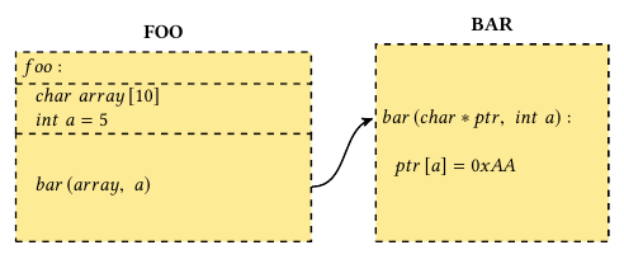
\includegraphics[width=\textwidth]{figures/cubicle_example_original.png}
         \caption{Original code of application FOO calling library BAR}
         \label{cubicleOriginal}
     \end{subfigure}
     \hfill
     \begin{subfigure}[b]{0.45\textwidth}
         %\centering
         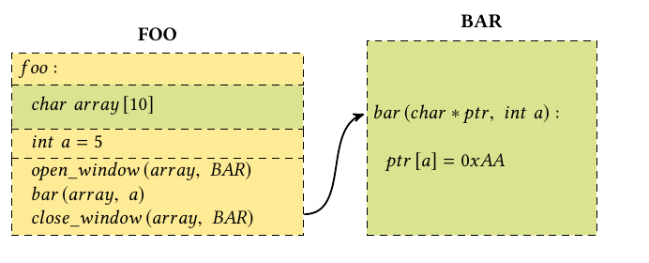
\includegraphics[width=\textwidth]{figures/cubicle_example_windows.png}
         \caption{Annotated code using Cubicles \textit{windows} to share memory after compilation}
         \label{cubicleWindow}
     \end{subfigure}
    \caption{To use Cubicle the developer basically needs to surround calls to other components, in this case BAR with \textit{windows}. Cubicle will derive isolated components and their (legitimate) interaction}
    \label{fig:CubicleAPI}
    \end{figure}

The aim of FlexOS~\cite{lefeuvre2021flexos} is to provide an easy way to exchange isolation primitives for existing code without (extensive) rewrites. Like CubicleOS it is based on an adapted version of the Unikraft library system. The two main primitives the FlexOS API provides are \emph{abstract gates} and \emph{abstract shared data}. In order to compile code with FlexOS, the programmer must replace all function calls between components with \emph{abstract gate} definitions and all shared memory areas with \emph{abstract shared data} definitions. These adjustments have also been made in the adapted system libraries. In addition the FlexOS build system needs a configuration file, which defines among other things the isolation mechanism and the division of the components. During compilation, the abstract definitions are replaced by concrete mechanisms of the target memory isolation techniques, which are MPK, Software Guard Extensions (Intel SGX) and Extended Page Tables \cite{intel64and}. 


In comparison to our approach, FlexOS and CubileOS solve a very similar problem with very similar constraints for the programmer. She has to define components and their communication explicitly and the adaptation to a concrete architecture is only possible through compilation, because she has to select from suitable system calls and libraries in the input already. In contrary to those systems, we do not provide an API to explicitly allow data sharing via references. It is possible to use reference sharing in Ohuas input programs, as only explicit reference passing is excluded. However Ohua will tread arguments passed by reference the same way as arguments passed by value. So if the resulting program is functional and if pass-by-reference is any more efficient than pass-by-value depends on the target architecture. Which also means we could not effectively use FlexOS or CubileOS as backend integrations.


\section{Compiling stateful imperative Programs to Data Flow}


"Making State Explicit for Imperative Big Data Processing"~\cite{fernandez2014making}:
\begin{itemize}
    \item identified problem: support arbitrary (Java) state in BigData (with high scalability) and recover state upon failure
    \item approach: infer dataflow and 'types of state access' to derive a 'stateful dataflow graph'(SDG)
    \item they explicitly focus on 'large states', where distribution of such state to several nodes is desirable both for performance/(storage/compute) capacity and for recovery after failure 
    \item SGD: "cyclic graph of pipelined data-parallel tasks, which execute on different nodes and access local in-memory state" \means no explicit scheduling
\item to identify 'partial' and 'partitioned' stateful objects, they require annotations from the programmer
\item they describe some concepts for parallel state handling and failure recovery, which might be helpful later
\item Graph derivation itself is not to fancy/smart \means  they require different annotations from the programmer to identify how particular states should be used (e.g. if they are global, mutable, can be partitioned etc), 
\item Limitiations:
\begin{itemize}
    \item programmer needs to annotate how states are used
    \item programmers need to implement the required primitives to handle state in the graph themselves (serialization, definitions for partitioning and recovery) or use predefined classes
    \item no side-effects on 'single valued' terms (marked by programmer), e.g. used as arguments for (stateful) computations
    \item deterministic execution: that's basically a requirement for sem. correct failure recovery e.g. program should not depend on current time or similar external state 
\end{itemize}
\item We do not aim to distribute the state handling itself, otherwise limitations/prerequisites are pretty similar
\item they work with checkpoints for failure recovery and synchronization of states and node replication (also for stateful nodes) to eliminate runtime bottlenecks \means not relevant for now, maybe later
\end{itemize}

"DFGenTool: A Dataflow Graph Generation Tool for Coarse Grain Reconfigurable Architectures "~\cite{mukherjee2017dfgentool}
\begin{itemize}
    \item generates a graph representation (DFG in DOT format) from a given program in LLVM IR \means advantages are obv. language+backend independence, but also that Basic Blocks are already identified and separated easing the conversion to nodes.
    \item available, though not maintained at \url{http://github.com/manideepam/DFGenTool}
    \item LLVM already provides SSA form, the guarantee that values are used only once and that copies are produced for values entering diverging control flow, also supported data types, by the looks of it are only int, float and arrays. Also to handle reassignments load and store dependencies are derived using LLVM alias analysis module
    \item \means maybe another example for easier scenarios but not helpful to get ahead, I might check how LLVM alias analysis module works though
\end{itemize}

"Automatic Extraction of Coarse-Grained Data Flow Threads from Imperative Programs" 
\begin{itemize}
    \item prototype compiler based on GCC for rec. C code
    \item only pure functions
    \item works on SSA representation
    \item interesting part: building program dependency graph from SSA (PDG), fuse strongly connected components (SCCs) using dependency analysis (simplified, eg. no arrays) \means "typed fusion", aligning dependency and data flow to data-flow-program-dependency-graph DF-PDG \means conversion algorithms     
    \item interesting also: mentions decoupled software pipelining (DSWP) technique \means Is it relevant for us?
\end{itemize}

\textbf{Automatically Restructuring Programs for the Web}~\cite{graunke2001automatically}
\begin{itemize}
    \item Caution: Paper is written in Scheme and in some parts badly abstracted from language features \means I might be wrong with some conclusions
    \item identified problem: 'traditional' (as in local, sequential, shared memory) interactive programs automatically save execution state during user interactions, but for interactive server applications developers need to implement this manually.
    \item paper presents (prototypical implemented) automated transformations, to turn a local interactive program into a CGI program
    \item the setting is (or is it?) slightly different from ours, as they also need to handle typical web interaction problems as duplicating browser windows (i.e. the entry points for interaction), back tracking user interactions a.s.o.
    \item Beside the 'you can port code easily' argument, they also argue as we do with better testing, debugging etc. of local code, being transformed to distributed only after the coding \means effectively they describe it as turning the program into a co-routine, with the other co-routine being the client. 
    \item Manual refactoring is described as we had done for egress/ingress i.e. every resume point after an interaction with the client (in our case the other components) becomes a function. The original main function now takes +1 input for every client call, specifying the entry point function.
    \item They mention an earlier approach to this, directly using continuations (cites 19 and 28 in the paper). The principle was that with Scheme, continuations could be derived and saved by the server automatically and assigned URLs, such that the client request can directly address the continuation. Problem was that this was a) language specific and b) had lots of overhead+distributed garbage collection 
    \item So the idea was to not store the continuation in the server, but embed it in the control flow
    \item For purely functional code transformation went as follows:
    \begin{enumerate}
        \item CPS: transform code to continuation passing style, i.e. make continuations explicit as arguments (I think, what we have are partial continuations)
        \item Lambda Lifting: Turn continuation expression into top-level functions (as for us everything happens inside a single state, they need not be separate functions but can just be blocks in the arms of matches ... Anyways it's not that different)
        \item Defunctionalization: Instead of passing the continuations as functions, a datatype/representation and an apply function are defined to a) represent a serializable (they say portable/can be marshaled) from of the functions b) interpret (actually the apply function is an interpreter isn't it?) the serialized functions to execute the corresponding code/continuation (concretely they derive a serializable structure for each lifted closure, capturing the required environment already when the form is send )
        \item[] The mention that, upon transformation to CPS "External modules that accept function arguments must be transformed as well."??? Why?
        \item The final step is, similar to us, to change semantics of prompting/asking for communication and control flow to according primitives for CGI ie. 'produce form' instead of prompting and looping to the beginning  if no continuation closure was returned.
    \end{enumerate}
    \item Note on \textbf{Security}: Instead of just passing input/output as in the original program, the derived program passes also information about the control flow inside the server/component. In this case, the whole continuation closures seem to be send. \means That is a good reason for dependency analysis i.e. do not send things, that do not belong to the other component \means but it remains a point that communication will leak execution state.
    \item for \textbf{stateful computations} they have the problem, that Scheme assumes call-by-value by default \means particularly relevant for lambda lifting
    \begin{itemize}
        \item so they introduce boxes (a way in scheme to share/call-by references), boxes for stateful values must be globally known
        \item they notice, that \emph{store} i.e. state changes are threaded through the program 'independent' from the control flow and needs to be saved between calls 
        \item so they basically save and retrieve the state as cookies and send them along. \means We do 'the same' but with less overhead, when we save selected parts of the execution to the state of our components. Reading and Setting cookies is in equivalent to getting and setting fields of the state before and after the execution of wrapped functions. Passing them between calls is implicitly done, because our \rust{apply} function is a method (\rust{process_call}).
    \end{itemize}
    \item one important distinction between our model and their application scenario is, that we do not assume the control flow to spontaneously divert e.g. by a client adding a second 'device' analogously to a second session tab in a browser. I'm not sure if/how that influences difference in our solution.
\end{itemize}

\textbf{Continuations from Generalized Stack Inspection}
\begin{itemize}
    \item a problem not addressed in CPS is the preservation of the run-time stack for "decomposed" functions
    \item there are languages like Scheme, that provide first-class continuations (i.e. they can be entirely send around) but most languages (in particular those running on VMs) do not provide means to programmatically save and reinstate the run-time stack. 
    \item One Solution was to move the run-time stack to the heap (there's just a sourceforge link in the bibliography :-( ), which is effectively what we did.
    \item The authors use a mechanism called \emph{continuation marks}. They are a form of stack inspection, enabling the programmer to attach values to the control flow stack and set marks, indexed by keys to the stack to later retrieve those values. In a first step they transform a Scheme program into this representation, in the second they use the marks to derive defunctionalization
    \item \means Not sure but this looks like deciding to integrate intermediate values into the data flow, while we decided to make them part of the local heap of stateful objects.
\end{itemize}


\textbf{Cooperative Task Management without Manual Stack Management
or, Event-driven Programming is Not the Opposite of Threaded Programming}~\cite{adya2002cooperative}
\means I think they also describe the transformations we are looking at, at least the part after components are inlined  but they explain it as a process from automatic to manual stack management
\begin{itemize}
    \item they bring some arguments and nice explanations for different concepts in
    concurrent programming in particular event-driven (cooperative tasks) vs. multi-threaded (preemtive or serial task management)
    \item event-driven is (according to the authors) easier to reason about concerning concurrent correctness
    \item anyways automatic stack management gets lost, bcs. it requires to dissect tasks, such that every subtask receiving an event (e.g. I/O in the original program) becomes a separate entry point \means this also means you loose big part of debugging info as the stack only tells you what happened since the last event came in
    \item 'Stack Ripping' is what they call the process of dissecting functions into basic blocks and making those callable functions \means each block containing an entry point after I/O (in our case after returning through the main loop), must become a 'language-level' function
    described required changes (same as we found out)
    \begin{itemize}
        \item function scope: more than one function now represent what was one function before \means trivial
        \item automatic variables: variables that where allocated on the stack, but need to survive multiple function calls now, needs to go to the heap \means been there, done that
        \item control structures: \means more entry points e.g. when looping \means more separate functions
        \item debug stack: manual recovery for manual stack management obviously
    \end{itemize}
    \item the rest of the paper explains how both types of stack management can be/are used together using cooperative scheduling in Windows (using threads and fibers respectively)
\end{itemize}

\textbf{Defunctionalized Interpreters for Programming Languages}~\cite{danvy2008defunctionalized}
\begin{itemize}
    \item loooots to unpack in this paper
    \item it build up on the works of Reynolds, Hutton, Kahn and many, many others in trying to complete a transformation relation among existing abstractions for computation. 
    \item the concrete transformation considered in the paper is that from \textbf{structural operational semantics} (including interruptions and errors) to \textbf{reduction semantics} using i) transformation to \textbf{continuation passing style} and ii) defunctionalization. 
    \item they integrate their results with previous work yielding the transformation based equivalence graph shown below (i.e. demonstrated inter-derivable representations)
    \item Given those results we can explore and maybe better describe in future what our transformations should be e.g. we could end up with defining stateful objects as abstract machines within the DFG (wild guessing )
\end{itemize}

\begin{figure}[H]
   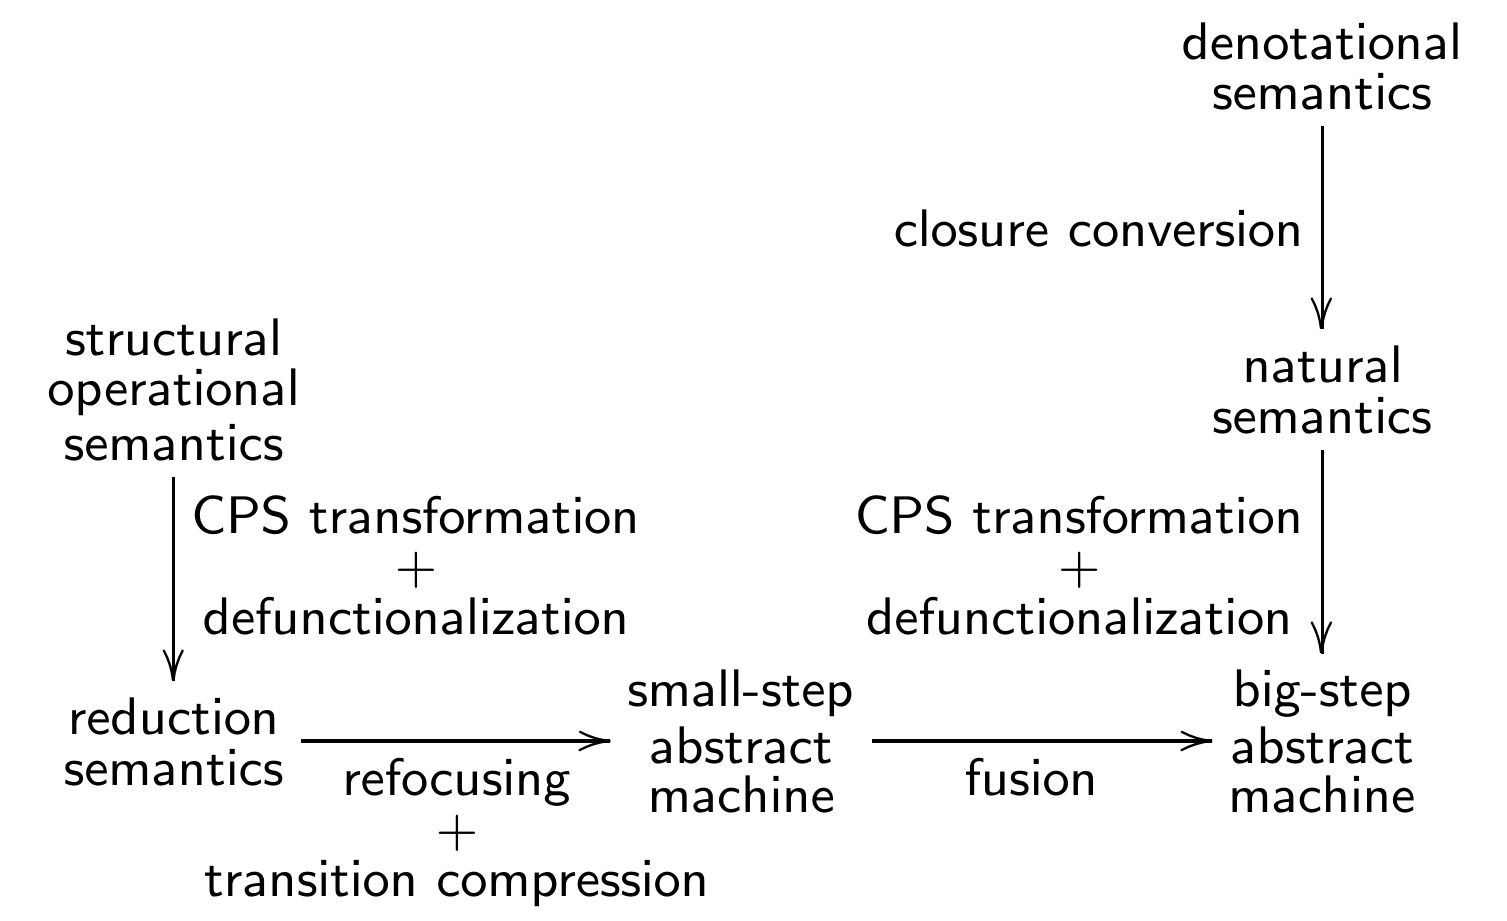
\includegraphics[width=\textwidth]{figures/transformations_danvy.png}
\caption{Graph representing the inter-derivability relation of different abstract models for computation, taken from Danvy~\cite{danvy2008defunctionalized}}
\label{fig:transformationsDanvy}
\end{figure}

\textbf{Refunctionalization at work}\cite{DANVY2009534}
\begin{itemize}
    \item in this paper, Danvy and Millikin present \textbf{Refunctionalization} the left inverse of Defunctionalization. 
    \item THis might be interesting for us, because this transformation as an intermediate step enables the transformations of programs that can not directly be fully defunctionalized. 
    \item As the authors notice "A program can fail to be in the image of defunctionalization if there are multiple points of consumption for elements of a data type or if the single point of consumption is not in a separate function.". This might be the case if we consider the transformation of \rust{poll}. 
    \item the two steps of deriving a common \rust{apply} function are called \emph{Disentangling} and \emph{Merging apply functions}.
    \item We should consider whether this helps us to formalize and generalize the transformations made in this work.
\end{itemize}
\todo[inline]{ I don't know where to put this so I don't forget, Danvys Dr.Sc. Thesis is titled "An Analytical Approach to Programs as Data Objects". Given the chapter titles I think its quite interesting and might be a good start to get the background for transformations}

Paper Stack Notes - Just for me now
\begin{itemize}
    \item Language-Agnostic Optimization and Parallelization for Interpreted Languages \means interesting is, that they don't use the language itself but analyze (static+dynamic) traces from the respective interpreters (with all problems that implies as having to separate interpreter introduced flow/dependencies from code flow/dependencies), they derive (or propose to do so) parallelity on the LLVM IR level
    \item Definitional Interpreters for Higher-Order Programming Languages \means very interesting for basic ideas (and wtf is GEDANKEN? Is it an actual language?), but for now to far off
    \item Software Compilation Techniques for
Heterogeneous Embedded Multi-Core Systems \means paper from our chair (at east Jeronimo is on the author list), point is that compilers for MPSoC should except sequential code for the same reasons we bring forward, same time the backend has to distribute parallel tasks in a more coarse grained fashion than single-core compilers do (ILP) \means maybe, if we come to the conclusion that atuomatic extraction of components is possible and stateful components should be annotated, why not annotate them with target architecture directive \means anyway that's just a (faaaarrrr) outlook perspective
\end{itemize}


Attempts to verify server-client programs (basically interaction of independent program components), some including stateful servers
\begin{itemize}
    \item "Towards reasoning for web applications: an operational semantics for Hop" 2010 \means defining small-step semantics for multi-tier programming language called Hop
    \item 'A theory of RPC calculi for client-server model' 2019 \means RPC calculus is from Wadler, to reason about web interactions, this paper extends it by stateful servers  
\end{itemize}

\section{Automatic memory Isolation}

\todo[inline]{Not sure if this belongs here but HAKC in particular the PhD thesis presents a technique to analyze function boundaries to isolate components \cite{mckee2022novel}, \cite{mckee2022preventing}. They also come to the rather obvious conclusion, that static analysis can not track pointers in general hence the do ...? to?}

 \textbf{HAKC}
 \begin{itemize}
     \item again the identified problem is lacking compartmentalization 
     \item in particular the authors make this case for Loadable Kernel Modules (LKM) which are themselves not a part of the linux kernel (i.e. not essential and not loaded by the bootloader), but loaded and executed in kernel space. With many of them providing audio and media processing and drivers, they are a notorious entry point for system compromise exploiting local bugs.
     \item HAKC provides an API to define componets and a hardware-baed runtime system to enforce in-kernel isolation of the defined components
     \item 
 \end{itemize}

 \textbf{FlexC} 
 \emph{Flex}ible \emph{C}ompilation is an approach to automatically generate the compartmentalization policies, that HAKC requires as interface definition in the Input code. The authors argue, that in particular in larger system hand-written annotations are error prone and might also lead to inefficient choices. Like HAKC itself, FlexC uses static information from the input code, to generate a data access graph from the input program. To account for indirect data access via pointers the analysis conservatively overestimates potential dependencies. Dynamic data i.e. test runs of the input code can additionally be provided to weighten the data dependencies by frequency of access and size of data. To start the derivation FlexC automatically assigns compilation units (in C usually one ore more files) as smallest entity of isolation. By defining the target number of compartments, the programmer can initialize a greedy fusion of nodes after the initial graph was build, generating a coarser compartmentalization. It is also possible to manipulate the graph using a GUI for FlexOS. The output of FlexC is then directly integrated to the compilation process using HAKC.


 \textbf{PKRU-Safe: Automatically Locking Down the Heap
Between Safe and Unsafe Languages}\cite{kirth2022pkru}
\begin{itemize}
    \item the identified problem is, that safe languages are already available and it should be possible to interact with unsafe language components without risking memory corruption
    \item So the whole point is to enforce hierarchic/semi-permeable memory isolation between Rust code and unsafe languages.
    \item the concept is 
    \begin{itemize}
        \item to have the developer explicitly define the interface between trusted and untrusted parts of the code, this is done via annotations in the projects build file and the untrusted libraries \means with per library annotations the adaptation overhead is significantly smaller than in annotating single functions or data access
        \item To analyse the code and track heap allocations PKRU-Safe uses custom plugins to rustc and LLVM tooling. To identify the usage sites of heap allocated data the input program is run with provided profiling input to dynamically identify when the untrusted component accesses data allocated by the trusted component.
        \item The gathered access data are used to categorize data allocation into unsafe and safe memory. At runtime this distinction is used to enforce the policy that unsafe code can never access safe memory.
        \item To move such data into the untrusted component entirely and to handle the two memory pools at run time the \rust{liballoc} to augment it by dedicated primitives for unsafe memory allocation. The authors describe this runtime behavior as \emph{compartment-aware} heap allocation. 
        \item By keeping heap section of safe and unsafe memory objects distinct, PKRU-Safe can implement the policies using MPK protection for the trusted heap section.
    \end{itemize}
    \item Stack data is assumed to be protected by other mechanisms (Shadow Stack [14, 40])
    \item they apply the concept to Servo, a layout-engine written in Rust. In the browser it interfaces with the JavaScript engine, written in unsafe C/C++ code.  
\end{itemize}
comparison
\begin{itemize}
    \item we will also need annotations for the components
    \item in fact if we implement the dependency analysis and make data part of the state we will achieve a similar effect. However we need to rely on the programmer not to implicitly share references.
    \item in how far data of one node is accessible to the other, depends on the backend and the programmers compliance to the programming model, not the compile process 
\end{itemize}


\textbf{Spons \& Shields}
\begin{itemize}
    \item a technique based on Intel SGX TEEs (Trusted execution environments)
    \item TEE are increasingly popular for secure cloud deployments and while they where initially used to encapsulate only specific critical user applications, they are now used to move whole OSes into a single secure environment e.g. into an Intel SXG enclave. 
    \item The identified problem is, again that this creates large code spaces without internal access restrictions and possibly including insecure, third party libraries, which contradicts the defense in depth approach.
    \item the next problem they notice is, that comparmentalization is often enforced along processes. But it is hard to redesign an application to encapsulate different concerns and security levels into different processes. Also the trust model of TEEs does not include the host, while process isolation techniques are based on the primitives the host OS and hardware (MMU) provide.
    \item they have a similar scenario as we do using an application containing an NGNIX, a PostreSQL (with medical data), an SSL library for crypto and a businesss logic application in PHP.
    \item The Spons\& Shields framework (SSF) described in the paper consists of an API to manage the two core abstractions \emph{Spons}, which encapsulate units of execution as POSIX processes or libraries and \emph{Shields} which define hierarchical memory access regions. The programmer needs to introduce \emph{Spons} and \emph{Shields} according to her requirements in the code and link against the musl standard C library. During compilation the framework will insert TEE primitives to enable the SSF runtime to enforce memory boundaries between the Spons.
    \item similar to our example they use a server-database scenario to exemplify their case (NGIX, PostgreSQL)
\end{itemize}
Comparison 
\begin{itemize}
    \item bound to C
    \item handwritten adaptations needed  
    \item maybe a backend ?
\end{itemize}



\todo[inline]{ Check \cite{9973038}: Combined approach using HW protection techniques, compile time analysis, model checking, and compiler runtime measures for protection. Probably cites a lot of approaches.}

\todo[inline]{ Abraham A Clements, Naif Saleh Almakhdhub, Saurabh Bagchi, and Mathias
Payer. ACES: Automatic compartments for embedded systems. In 27th USENIX
Security Symposium (USENIX Security 18), pages 65–82, Baltimore, MD, Au-
gust 2018. USENIX Association.
}